% !TeX root = DistributedConsensus.tex
% !TeX spellcheck = en_GB
\chapter{Connecting Histories}\label{chap:connecting-histories}
	After determining how to represent histories, we want to combine multiple histories into one history using the information of actions.
    
    \section{Merging Histories}\label{sec:connecting:merge}
    Having defined the representation of history, and the fact that the actions of executions are distributed among several events, we need a way to connect the actions by happens before relations.

	\newpar In order to simplify this problem it is assumed that all local histories are \textit{\textbf{valid}}. That is:
    
    \begin{definition}
    A \textit{\textbf{valid history}} is a history, where all actions happen according to the rules of the DCR graph, abiding serial equivalence and being in strict partial order. Also, a valid history \textbf{must} contain exactly the actions that \textbf{did} happen in the execution of events.
    \end{definition} 

	\noindent The observation and identification of invalid histories are described in \autoref{chap:validation}. Why it is necessary to have this assumption is discussed in the end of this section.

    \newpar Given valid local histories of several events, we want to connect the actions of the histories such that the result has the fewest possible concurrent actions using happens before relations. Furthermore, given a global history $A$ and every local history $B$ used for the creation of $A$, for every path from action $x$ to another action $y$ in $B$, there must also exist a path from $x$ to $y$ in $A$.
    
    \newpar We will use the local histories in \todo[backgroundcolor=green]{Indsæt figur som er input til merge algoritmen.} as an example for the remainder of this section.
    
    \newpar The concept of happens before relations, as described in \autoref{subsec:orderingofevents} helps determining which actions have happened before others across events. For each outgoing action in a history, there must be another incoming action, because these actions are the two sides of the same effect. Therefore, each outgoing action type corresponds to an incoming action type by the following definition:
	
	\begin{definition}
		\label{def:happensbeforeaction}
		The action types that \textbf{correspond} are:
			\begin{itemize}
				\item Checks condition $\rightarrow$ Checked condition by
                \item Excludes $\rightarrow$ Excluded by
				\item Includes $\rightarrow$ Included by
				\item Sets pending $\rightarrow$ Set pending by
			\end{itemize}
	\end{definition}
	
	\noindent For any outgoing or incoming action on an event, there might exist any number of actions with corresponding action types. Actions should therefore be matched on more than just their corresponding action type. An action includes the ID and timestamp of both the executing and counterpart event to ensure that matches are unique.
    Pairs of actions \textbf{\textit{match}} if they share a corresponding type, while the ID and timestamp of either action matches the counterpart ID and timestamp of the other.
    
    \begin{definition}
    	\label{def:action:matching}
    	A pair of actions, $a$ and $b$, \textit{\textbf{match}} if and only if they have corresponding action types and the ID and timestamp of $a$ is identical with the counterpart ID and counterpart timestamp of $b$. Furthermore, the ID and timestamp of $b$ must be identical with the counterpart ID and counterpart timestamp of $a$.
    \end{definition}
    
    \noindent Figure \ref{fig:connect:actions-match} is an example of a pair of matching actions.  In \autoref{fig:connect:actions-do-not-match} the actions do not match.
    
    \begin{figure}[H]
		\centering
		\begin{minipage}{0.45\textwidth}
			\centering
			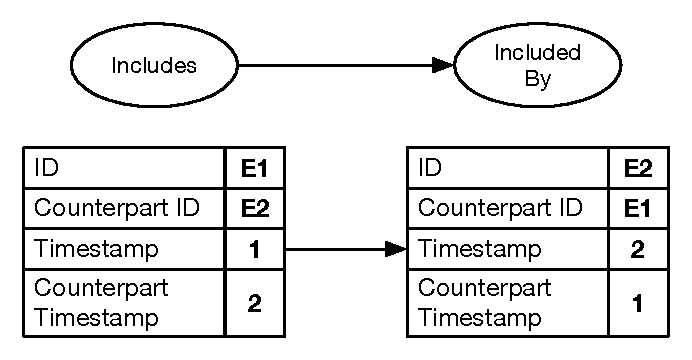
\includegraphics[width=\textwidth]{4connect/images/actions-match.pdf}
			\caption{Two actions that match.}
			\label{fig:connect:actions-match}
		\end{minipage}\hfill
		\begin{minipage}{0.45\textwidth}
			\centering
			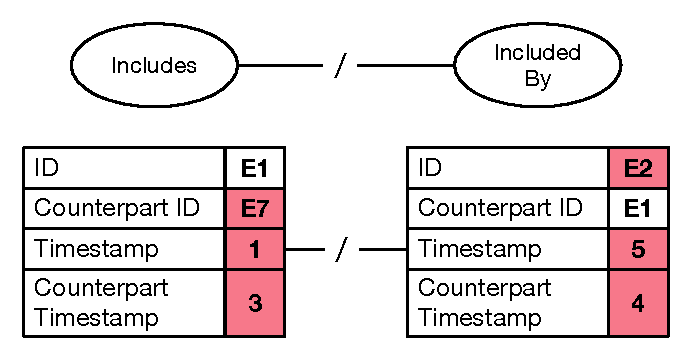
\includegraphics[width=\textwidth]{4connect/images/actions-do-not-match.pdf}
            \caption{Two actions that do not match. Fields that do not match are marked with red.}
            \label{fig:connect:actions-do-not-match}
		\end{minipage}
    \end{figure}
        
    \noindent An outgoing action must happen before its incoming counterpart, because together they represent a message exchange between to processes. A happens before relation is established between the matching actions. Therefore an edge can be added from the outgoing action to the incoming action in a history.

	\newpar To create a history of the entire set of events, every action of every local history needs to be added to a joined history. Whenever a pair of matching actions are found, the edge is added from the outgoing action to the incoming action. With this algorithm a set of histories can then be merged together, two at a time, until one final combined history remains. The \textit{Merge} algorithm is outlined in \autoref{alg:merge}.
	
	\begin{algorithm}
		\begin{algorithmic}
			\Function{Merge}{history1, history2} \textbf{returns} \textit{a merged history}
			\State combinedHistory $\leftarrow$ \Call{UnionNodesAndEdges}{history1, history2}
			\ForAll{action \textbf{in} combinedHistory}
			\If{\Call{IsOutgoing}{action}}
            	\ForAll{action' \textbf{in} combinedHistory}
                	\If{\Call{Matches}{action, action'}}
						\State combinedHistory $\leftarrow$ \Call{AddEdge}{action, action', combinedHistory}                    	
                    \EndIf
                \EndFor
			\EndIf
			\EndFor
			\State\Return combinedHistory
			\EndFunction
		\end{algorithmic}
		\caption{The \textit{\textbf{Merge}} algorithm}
		\label{alg:merge}
	\end{algorithm}
	
    \noindent Figure \ref{fig:connecting:match-before-after} shows the histories of two events, before and after a matching pair of actions have been found.
    
	\begin{figure}[H]
		\centering
		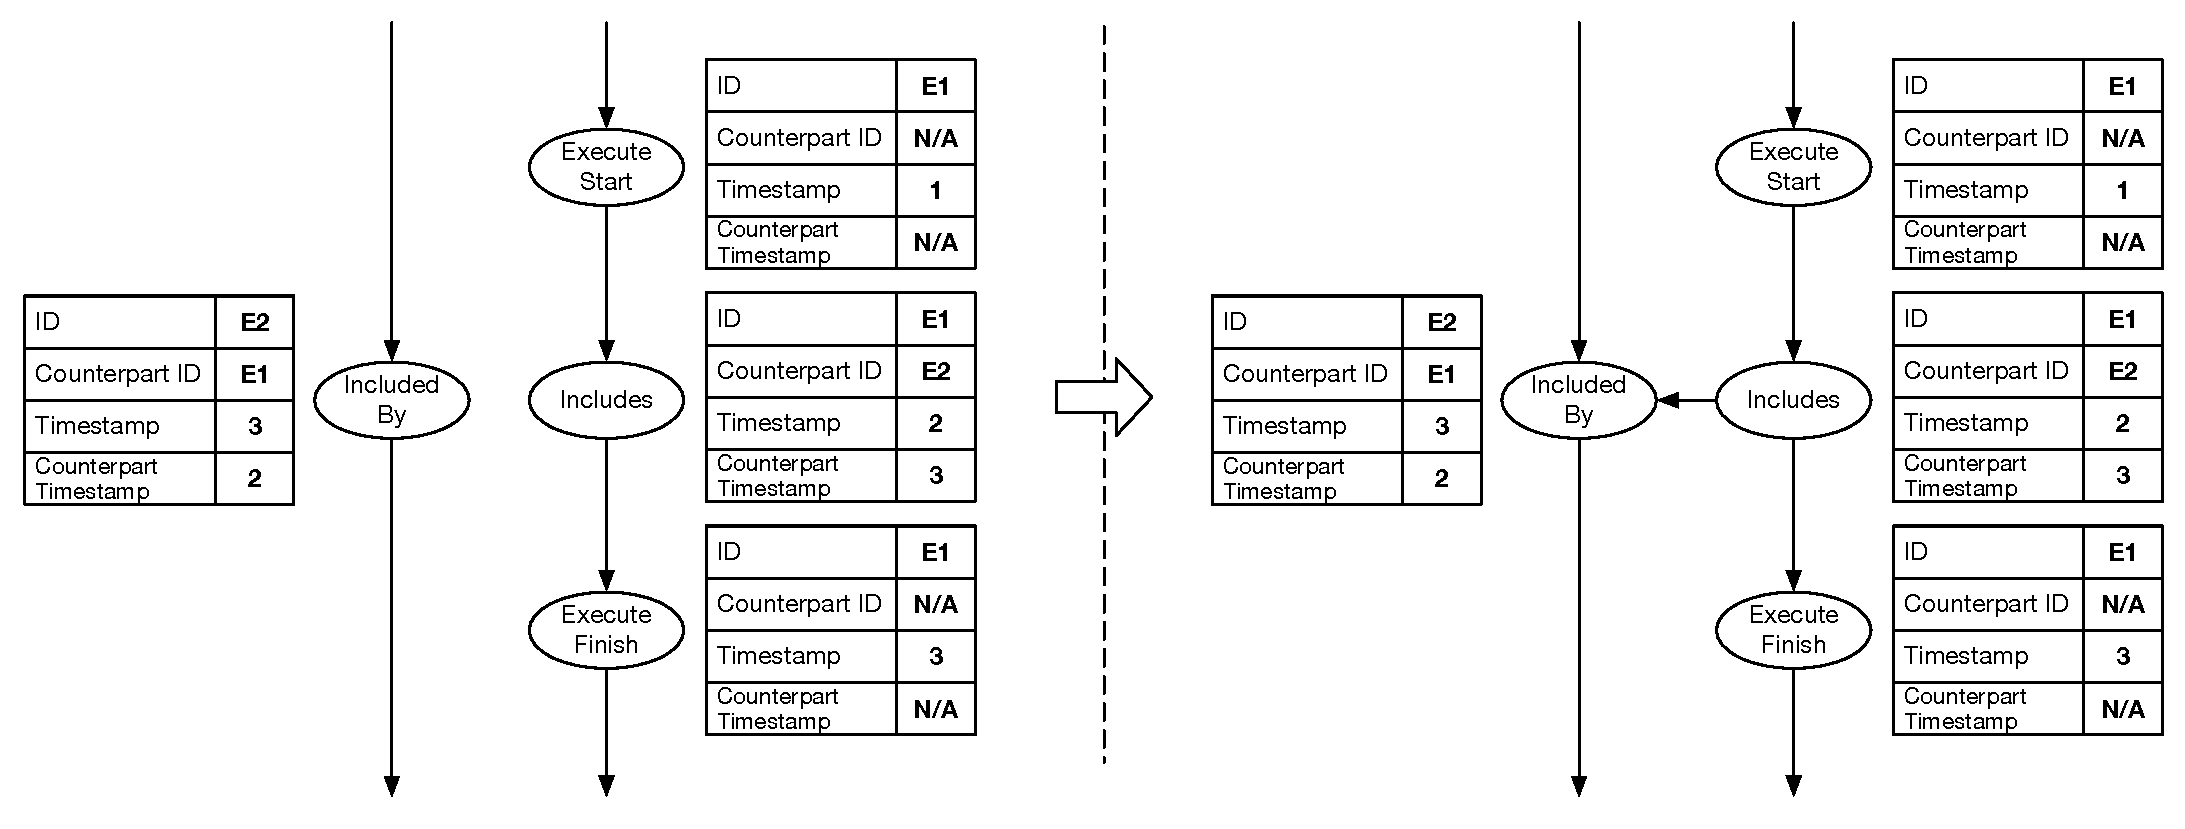
\includegraphics[width=\textwidth]{4connect/images/match-before-after.pdf}
		\caption{Actions of two merged histories before and after being matched.}
		\label{fig:connecting:match-before-after}
	\end{figure}
	
    \subsection{Correctness}
    In order to show that we have solved the problem of merging histories, we must show that all existing happens before relations of the local histories are still preserved and that we have added all of the possible happens before relations across histories.\todo{Er possible godt nok?}
    
    \newpar Since the method takes the union of all of the histories, which implies the union of all the action sets and happens before sets, and because no actions or happens before relations are removed, all the existing actions and happens before relations are preserved in the global history, which means that all paths in the local histories are present in the global history.
    
    \newpar Given that the union of all local histories contains the actions of every message exchange that has happened in the workflow and we have found all matching actions, corresponding to every message exchange, then every message exchange must be part of the global history. Because we can only find happens before relations across processes when they have exchanged a message, we have found all happens before relations between events.
    
    \newpar If we do not assume that all local histories are valid, it is not possible to assert that the union of the local histories contains all the actions and happens before relations between the actions that have happened, and therefore the global history will not be a representation of the actual global history of the workflow. This also means that we cannot assert that message exchanges, and actions in general, are not created, omitted, or changed. In the end, the algorithm would return an invalid global history if we do assume that all local histories are valid.
    
    \todo[inline]{Måske noget med at vi pga. dataen ikke kan gøre noget ved dette.}
    
    \section{Gathering of History}
    To merge the histories together it is necessary to acquire the local histories of the events of the DCR graph. In a central server system where the server has access to all the individual events it is a trivial task to gather the histories. Simply request the server to get access to all the events and then request the histories of each event individually. This method is simple and only relies on the central server to get the addresses of all the events in the workflow. Furthermore the amount of messages sent to recieve all histories is $2N+2$ where N denotes the amount of events in the system. An illustration of this architecture is shown on \autoref{fig:connecting:server-contacts-events}.
    
    \begin{figure}[H]
    	\centering
    	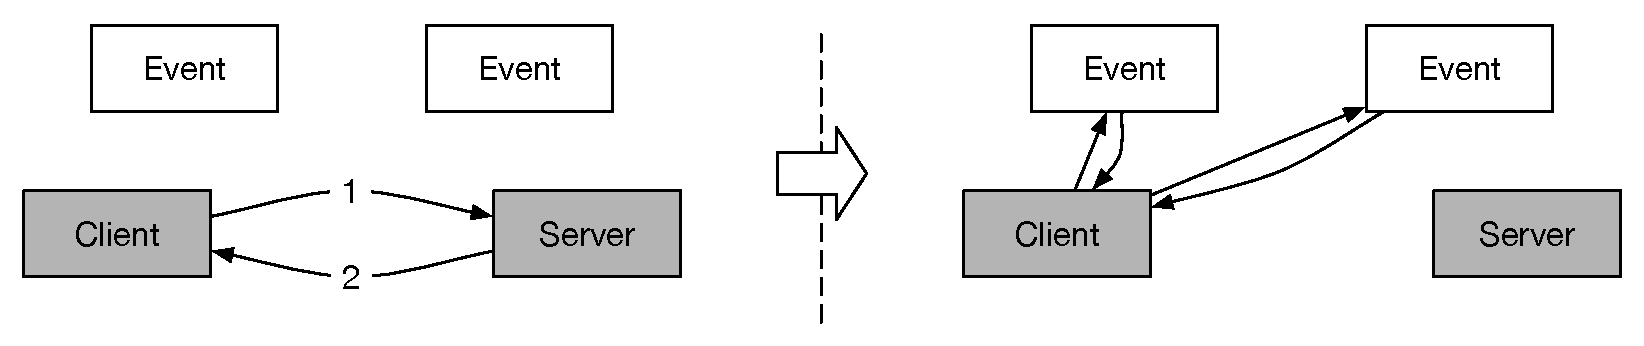
\includegraphics[height=\textheight/6]{4connect/images/server-contacts-events.pdf}
    	\caption{The client requesting history from events and receiving it.}
    	\label{fig:connecting:server-contacts-events}
    \end{figure}
    
    \newpar Unfortunately, central server systems have drawbacks. E.g. if the server crashes then it is not possible to acquire the addresses of any of the events and the server has to do the entire workload instead of distributing it out across the peers.\todo{Mikael: Jeg er med på den første del af denne sætning, men forstår ikke resten.}
    
    Therefore it could be desirable to create a peer to peer-based gathering algorithm, but this introduces a new set of challenges.
    
    \subsection{Gathering Without a Central Server}
	Presumed that it is desired to know nothing about the distribution events in the DCR graph, and therefore have no central all-knowing server handling gathering of history, an alternative approach of gathering history using recursive traversal of the DCR graph can be developed. The following section describes this approach, and the shortcomings of it. 
	
	\newpar In order to gather history from a given workflow using recursive traversal, a single starting event must be known. The reachability of this event should preferably be the set of all other events in the workflow. If the reachability is a subset of all the events, then only a subset of all the local histories of the events can be gathered. Therefore the greater the reachability of the beginning event, the more complete the gathered history will be. It can therefore not be guaranteed that history from every event will be gathered if the DCR graph is not fully connected. This constitutes the first drawback of this approach.
	
	It is desired to develop an algorithm that, given an event with the desired reachability, is able to recursively gather all the local histories of the workflow. Since DCR graphs can contain cycles the algorithm also has to avoid endless recursions.
		
	\subsubsection{The Produce Algorithm}
	Given a DCR graph where all events are reachable from the starting event, the algorithm should gather and merge the histories of each event in the graph into one global history.
	
	This is accomplished by recursively contacting neighbouring events and asking them for their history while merging the neighbours' histories with its own history. To handle cycles, the use of a \textit{trace set} of previously contacted events is sent from each event to the next.
	
	\newpar The implementation of this solution uses two sets, called \texttt{request trace} and \texttt{wait for}, which is used for tracing and cycle avoidance respectively. The algorithm propagates throughout the graph using recursion while avoiding infinite cycles of requests. 
	
	When an event receives a request for its history, it adds every neighbouring event to \texttt{wait for}, and \texttt{request trace} set is subtracted from the \texttt{wait for} set. If the \texttt{wait for} is the empty set, the history of the event is returned. If \texttt{wait for} is not empty the event sends requests to all events in \texttt{wait for} with its own ID appended to the \texttt{request trace}. When the event receives histories from its neighbours, it merges the histories and returns the merged history to the requester. The algorithm can be seen in \autoref{alg:produce}. A run of the produce algorithm is illustrated in \autoref{fig:connecting:recursive}.
	
	\begin{algorithm}
	\begin{algorithmic}
		\State Event receives request for history with a \texttt{request trace}, $T$.
		\State Event has internal \texttt{wait for}, $W$
		\State
		
		\Function{Produce}{T, W, event}
			\State $W\gets$ \Call{Union}{$W$, event.Neighbours}\Comment Add all neighbouring events to \texttt{wait for}.
			\If {$W=\emptyset$}
				\Return own history
			\Else
				\State $W\gets$\Call{Minus}{W, T}\Comment Remove every event in $T$ from $W$. Cycles avoided.
				\State $T'\gets$\Call{Append}{event.Id, T}\Comment Append own event ID to $T$.
				\State
				\ForAll {$w$ in $W$} 
					\State request history from $w$ with $T'$
				\EndFor
				\State wait for receiving histories
				\State merge received histories with own history
				\State
				\Return merged histories
			\EndIf
		\EndFunction
	\end{algorithmic}
	\caption{The \textit{\textbf{Produce}} algorithm}
	\label{alg:produce}
	\end{algorithm}\todo{Mikael: Er wait for ikke altid det samme som naboerne? Jeg har i øvrigt forsøgt at gøre det lidt mere pseudo end f\#}
		
	\begin{figure}[H]
		\centering
		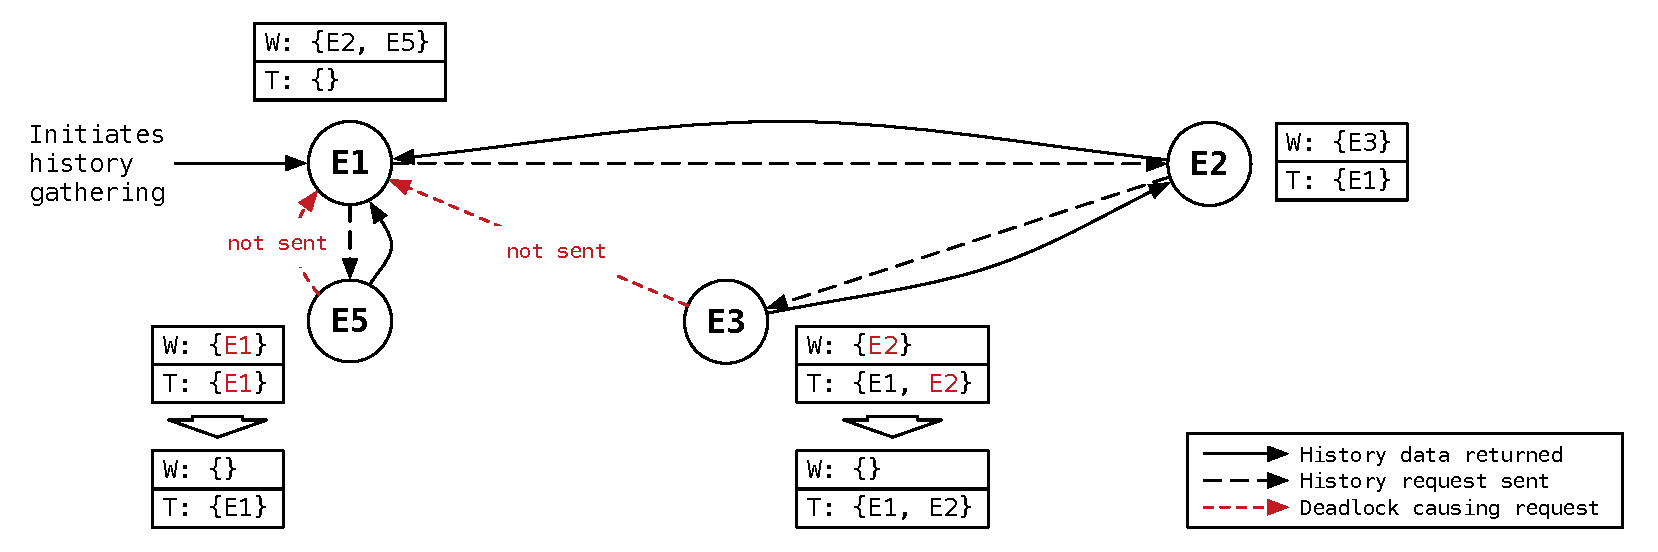
\includegraphics[width=\textwidth]{4connect/images/recursive.pdf}
		\caption{An illustration showing the recursive traversal through a graph. Note the avoidance of creating a deadlock.}
		\label{fig:connecting:recursive}
	\end{figure}
		
	\newpar This algorithm is in fact a modified version of the \textit{flooding search algorithm} \todo{Kapitel 6, side 250 distributed bog} for searching in unstructured peer to peer networks. Contrary to the flooding algorithm, the produce algorithm not only returns the value at the searched for node, but returns every value at every reachable node. The flooding algorithm is often implemented with a time limit on the search and therefore does not care about cycles, which is handled more efficiently in the produce algorithm. Furthermore in the produce algorithm, every path to a node returns the value of that node. 
	
	\subsubsection{Correctness}
	To argue that the produce algorithm correctly gathers all the local histories in the workflow we must show that every event is contacted. Since the algorithm takes the neighbour of every contacted event, and the beginning event has a reachability of every event in the workflow, the set of contacted events must be all events in the workflow. If it is assumed that every event returns their history, as well as any recursively contacted event, then every history of the workflow must be returned to the beginning node. 
	
	The assumption that every event returns the history of every recursively contacted event, is unsafe in systems with Byzantine errors.
	
	\subsubsection{Issues with Recursive Traversal of the Distributed Graph}
	\todo[inline]{Omformulér afsnit om, at det er tæt på umuligt at validere historik (specielt vha. DCR-regler) uden at kende hele workflowet.}
	
	If malicious processes are introduced in the DCR graph, the problem similar to not having full reachability from the beginning event arise. If the path to a given event, goes through an event on a malicious process, then that malicious process can either add, remove or change the history. That implies that any history retrieved from that event, might not be valid. The effects of this malicious behavior is worsened if the event is reached early on during the gathering. An illustration of this is shown in \autoref{fig:connecting:recursive-evil-node}. If there exists no path to an event that does not go through a malicious process, then the beginning node will potentially not have any valid version of that history. Even if it is possible to assert that the history is invalid, it is not possible to identify which event along the path has acted maliciously.
	
	\newpar That is, if the neighbouring events do not know enough of each other, there is no way of making sure that the returned history is correct. Furthermore, this uncertainty is amplified due to the fact that for each contacted event with lacking information, it is possible to tamper with the history of the recursively called events, or even add history of non existent events. Therefore some action must be taken to handle these pitfalls.
	
	The requirements for making it possible to validate the gathered history are described in the following section. 
	
	\begin{figure}[H]
		\centering
		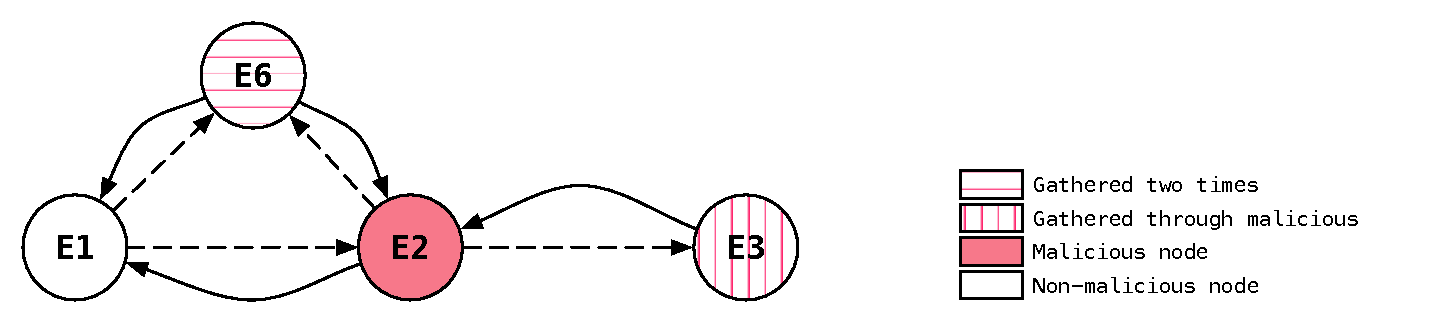
\includegraphics[width=\textwidth]{4connect/images/recursive-evil-node.pdf}
		\caption{A malicious node in a graph. Note that it is not possible to ensure that any history passing through the malicious node is valid.}
		\label{fig:connecting:recursive-evil-node}
	\end{figure}
	\todo[inline]{Mikael: Det er lidt mærkeligt at det øverste E2 også er farvet delvist rødt?\\Fisk: Den er delvist farvet, da den kan være fucked up, hvis E1 får historik fra den via E2. Slutteligt skal vi slef. lige sige, at denne algoritme derfor ikke er anvendt.\\Mikael: Men man får jo både historikken fra E6 og E2, men du har nok ret.}
	
	\subsubsection{Performance}
	This algorithm has a worst case message performance is exponential. \todo{Fisk: What?} This is due to the want to have redundant history every path from a given node to any other reachable node needs to be examined. The worst case is when the graph is fully connected and every node therefore has a node to any other node. High connectivity in the graph is a wanted property since it allows for better validation of the histories. \todo{Fisk: Måske uddyb hvorfor dette er tilfældet? Eller i hvert fald så kæde sammen med nedenstående?}
	
	\newpar Caching history produced of an event before transferring it to a requesting event could improve performance, but presents new problems. 
	
	Certain issues arise if an event with neighbours is the last event in what would have been a produce cycle and due to tracing returns its own local history which would then be cached. This event would then never return the histories of its neighbours if contacted again from a different event, but would instead only return its own history due to caching. 
	
	The neighbours history of the neighbours would then only be produced once, and therefore pass through a single, possibly malicious, node. The lack of redundancy in the system therefore presents an issue when validating histories.
	It is therefore necessary to produce redundant histories, which makes caching impossible.\todo{Vi snakkede om med søren på et tidspunkt at vi også hellere ville exploite DCR end at gøre det distribueret, og at der var flere muligheder for at snyde ved at gøre det på denne måde.}